\documentclass[conference]{IEEEtran}
\IEEEoverridecommandlockouts
\usepackage{amsmath,amssymb}
\usepackage{graphicx}
\usepackage{booktabs}
\usepackage{array}
\usepackage{xcolor}
\usepackage{tikz}
\usetikzlibrary{positioning,arrows.meta,fit,backgrounds}
\usepackage{url}
\usepackage[hidelinks]{hyperref}

\newcommand{\tool}{\texttt{dc-profile}}

\begin{document}

\title{AI Demand Controller for Resource-Aware Diagnostic Evidence Delivery in Codebase Tuning: A Pre-Registered Pilot}

\author{\IEEEauthorblockN{Gowtham Balasubramanian}
\IEEEauthorblockA{Email: gowthamkopite@gmail.com}}

\maketitle

\begin{abstract}
Coding agents asked to make a repository faster need to know where time is
spent, but profiler output is costly to collect and can be far longer than
what an agent can usefully read. A \emph{demand controller} sits between the
agent and the profiler: it admits profiling requests against a fixed
allowance, shows the remaining allowance after each call, and returns a
compressed artifact instead of the raw profile. Profiler-guided agents and
cost-aware profiling harnesses already exist, so the idea itself is not new.
This paper makes a narrower contribution: a controlled, pre-registered pilot
that compares evidence \emph{formats} at a fixed allowance. We compare no
profiler tool, a truncated raw cProfile listing, and a ranked hotspot table,
with the meter kept on the host where the agent cannot alter it, and we
measure whether the agent uses the tool at all. The pilot uses 18
SWE-fficiency tasks from 8 Python repositories, one fixed agent and model, and
one run per task and condition. The agent almost never used the tool. One of
18 runs in each tool condition called it, both calls failed, and no agent in
the pre-registered set received a profile. Runs took 1.5 minutes on average.
The pre-registered overall scores were 0.038 (95\% CI 0.014--0.559) with no
tool, 0.038 (0.014--0.567) with the dump, and 0.036 (0.013--0.386) with the
ranked table. These scores are dominated by one task whose expert patch fails
required tests on our machine. An audit found such failures on 7 of 18 tasks,
and 10 of 54 predictions went unscored because of infrastructure errors. In
the secondary analysis of all 32 tasks with complete runs, every paired
difference has an interval that includes zero. The pilot therefore says
nothing about evidence format. Its value lies in the problems it exposes for
a larger study.
\end{abstract}

\begin{IEEEkeywords}
LLM agents, performance profiling, budget-aware tooling, code optimization,
tool output compression, pre-registration
\end{IEEEkeywords}

\section{Introduction}

Large language model (LLM) agents can now read a repository, edit it, and run
its tests inside a container~\cite{yang2024sweagent,xia2024agentless}, and
benchmarks such as SWE-bench measure whether they resolve real
issues~\cite{jimenez2024swebench}. A large literature now studies LLMs for
software engineering~\cite{hou2024llm4se}.
Performance work is harder. The agent must keep behaviour unchanged while
making a given workload run faster, and the place where time is spent is
often not obvious from the code. Recent benchmarks built from real
performance-improving commits, namely SWE-fficiency~\cite{ma2025swefficiency},
GSO~\cite{shetty2025gso} and SWE-Perf~\cite{he2025sweperf}, report that agents
reach only a small fraction of expert speedups. The GSO and SWE-fficiency
authors list poor localization of bottlenecks among the main failure modes.

A profiler is the standard tool for localization, but giving an agent a
profiler is not free. First, profiling costs wall-clock time that the agent
could otherwise spend editing and testing. Second, a full profile of a library
call can list thousands of functions. Long tool outputs fill the context
window, and models use information in the middle of long contexts less
reliably~\cite{liu2024lost}. Third, a profile can mislead: profilers can
attribute time to the wrong function~\cite{mytkowicz2010evaluating}, and the
function that takes the most time is not always the one whose optimization
shortens end-to-end runtime~\cite{curtsinger2015coz}.

We call the layer that manages this trade-off a \emph{demand controller}. It
decides whether a profiling request is admitted, charges it against a visible
allowance, and returns a compressed artifact rather than the raw profile.

\textbf{This idea is not new.} PerfAgent~\cite{deng2026perfagent} gives an
off-the-shelf agent curated hotspot summaries from a sampling profiler,
re-profiles after each patch, and runs selective tests, and it reports large
gains on GSO and SWE-fficiency-Lite. ProfileWeaver~\cite{ding2026profileweaver}
describes a cost-aware controller that selects profiling actions under token,
time and iteration budgets and normalizes the results of several profilers
into a shared hotspot summary. What
these systems do not isolate is the effect of the evidence \emph{format}.
They bundle the profiler with loop control, verification and other changes,
and they do not report whether a ranked summary beats a plain truncated dump
when everything else is held fixed.

This paper asks a narrow question. At a fixed allowance of profiler calls,
does a ranked hotspot table help a coding agent more than no profiler tool or
a truncated raw profile, and does the agent use the tool at all? Our
contributions are:
\begin{itemize}
\item A small demand controller whose meter runs on the host as an HTTP
  service, so the agent inside the task container cannot read or reset it
  (Section~\ref{sec:design}).
\item A pre-registered pilot on SWE-fficiency that varies only the evidence
  format (none, truncated dump, ranked table), with the task sample,
  replacement rule, metrics and every amendment committed to git before the
  runs they affect (Section~\ref{sec:method}).
\item Measurements of tool use: how often agents call the profiler, run into
  the allowance, or profile on their own through the shell. These numbers
  matter because a format cannot help if the agent never asks for it
  (Section~\ref{sec:results}).
\item An audit of every run and score, which shows how emulation, memory
  limits and the correctness oracle can decide a small study's result.
\end{itemize}

\section{Related Work}

\textbf{Benchmarks for repository-level optimization.}
SWE-fficiency~\cite{ma2025swefficiency} contains 498 tasks from nine Python
repositories. Each task gives the agent a repository and a slow workload, and
scores the patch by the \emph{speedup ratio}: the agent's speedup divided by
the expert patch's speedup, aggregated across tasks by a harmonic mean. Patches
that fail the selected unit tests count as incorrect. GSO~\cite{shetty2025gso}
generates performance tests from commit histories across ten codebases in
several languages. SWE-Perf~\cite{he2025sweperf} uses 140 instances from
performance-improving pull requests. Earlier work on program-level
optimization, such as PIE~\cite{shypula2023pie}, studied performance-improving
edits to single programs rather than whole repositories. We build on
SWE-fficiency because its harness, workloads and agent prompt are released and
it scores against expert patches.

\textbf{Profiler-guided agents.}
PerfAgent~\cite{deng2026perfagent} is the closest prior work. It collects
py-spy samples, filters setup frames, aggregates them into hotspots with self
time, total time and call context, re-profiles after every submitted patch,
and runs only the tests affected by the change. Its authors note that agents
left alone often skip profiling or use Python's built-in cProfile, which has
high overhead and does not see inside native extensions.
ProfileWeaver~\cite{ding2026profileweaver}, published as a poster, wraps
several HPC profilers as skills with an expected insight and acquisition cost.
Its controller selects actions by expected insight per unit cost under token,
time and iteration budgets. Our controller is a much simpler version of the
same idea. The difference is the experimental design: we hold the agent,
prompt, allowance and profiler fixed and change only the rendering.

\textbf{Tool-output compression.}
Coding agents read long tool outputs, and only a small part of each output
matters for the next step. Squeez~\cite{kovacs2026squeez} trains a small model
to prune tool output to the evidence block the agent needs. SWE-agent showed
that the design of the agent--computer interface, including how command output
is shown, changes agent success~\cite{yang2024sweagent}. A ranked hotspot table
is a hand-written, domain-specific compressor of this kind.

\textbf{Profiler accuracy.}
Profiles are evidence, not ground truth. Different Java profilers can disagree
on the hottest method because of where they sample~\cite{mytkowicz2010evaluating}.
Causal profiling~\cite{curtsinger2015coz} shows that the time spent in a
function can differ from the gain available by optimizing it. Flame
graphs~\cite{gregg2016flame}, the usual way engineers read stack profiles,
are visual and do not fit a text-only agent interface.

\section{Demand Controller Design}
\label{sec:design}

\textbf{Model.} A tool $T$ maps a program $P$ and workload $W$ to an evidence
artifact $E=T(P,W)$. The agent reads $E$ and produces a patch $\Delta$, which is
scored by correctness and speedup. In general the controller holds a budget
$B=(A_{\max},T_{\max},K_{\max})$ on profiler calls, profiling time, and evidence
tokens, and admits a request only if its cost fits the remaining budget. The
pilot implements only the first component: a limit of four calls per task.
Profiling time is not metered separately. It comes out of the agent's 30-minute
wall-clock limit, so no condition receives extra time. Token cost is bounded by
the format.

\begin{figure}[t]
\centering
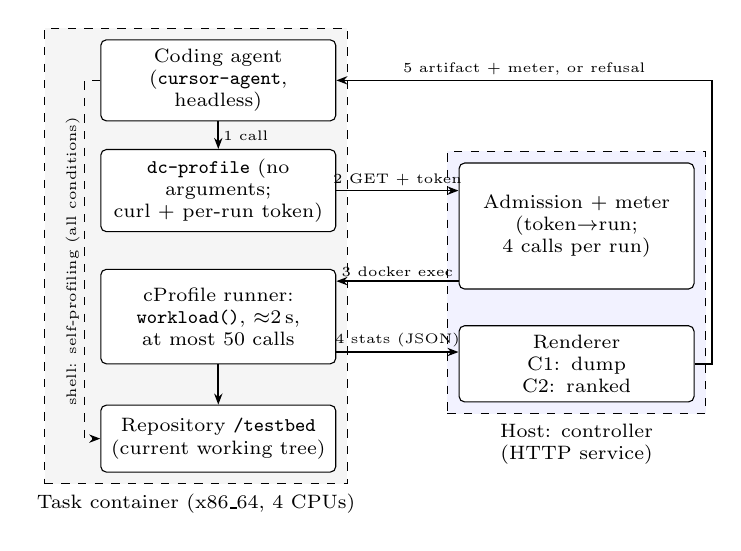
\begin{tikzpicture}[
  font=\scriptsize,
  box/.style={draw, rounded corners=2pt, align=center, text width=2.75cm,
              minimum height=0.85cm, fill=white},
  arr/.style={-{Stealth[length=4pt]}, semithick},
  lab/.style={inner sep=1.5pt, font=\tiny}]
  \node[box] (agent) at (0,0) {Coding agent\\(\texttt{cursor-agent}, headless)};
  \node[box] (cli)   at (0,-1.4) {\tool{} (no arguments;\\curl + per-run token)};
  \node[box, minimum height=1.2cm] (prof) at (0,-3.0)
        {cProfile runner:\\\texttt{workload()}, $\approx$2\,s,\\at most 50 calls};
  \node[box] (repo)  at (0,-4.55) {Repository \texttt{/testbed}\\(current working tree)};
  \node[box, minimum height=1.6cm] (adm) at (4.55,-1.85)
        {Admission + meter\\(token$\to$run;\\4 calls per run)};
  \node[box] (rend)  at (4.55,-3.6) {Renderer\\C1: dump \quad C2: ranked};
  \node[rotate=90, font=\tiny] (selflab) at (-1.85,-2.3) {shell: self-profiling (all conditions)};
  \coordinate (y2) at (0,-1.4);
  \coordinate (y3) at (0,-2.55);
  \coordinate (y4) at (0,-3.45);
  \begin{scope}[on background layer]
    \node[draw, dashed, fill=gray!8, inner sep=4pt, fit=(agent)(repo)(selflab),
          label={[font=\scriptsize]below:Task container (x86\_64, 4 CPUs)}] {};
    \node[draw, dashed, fill=blue!5, inner sep=4pt, fit=(adm)(rend),
          label={[font=\scriptsize, align=center]below:Host: controller\\(HTTP service)}] {};
  \end{scope}
  \draw[arr] (agent) -- node[lab, right] {1 call} (cli);
  \draw[arr] (cli.east |- y2) -- node[lab, above] {2 GET + token} (adm.west |- y2);
  \draw[arr] (adm.west |- y3) -- node[lab, above] {3 docker exec} (prof.east |- y3);
  \draw[arr] (prof.east |- y4) -- node[lab, above] {4 stats (JSON)} (rend.west |- y4);
  \draw[arr] (prof) -- (repo);
  \draw[arr] (rend.east) -- ++(0.22,0) |- node[lab, pos=0.75, above] {5 artifact + meter, or refusal} (agent.east);
  \draw[arr, dashed] (agent.west) -- ++(-0.2,0) |- (repo.west);
\end{tikzpicture}
\caption{Demand controller used in the pilot. The meter and renderer run on
the host, so the agent cannot change them. In every condition the agent can
also profile through its own shell (dashed).}
\label{fig:arch}
\end{figure}

\textbf{Pipeline.} The controller has four stages (Fig.~\ref{fig:arch}).
\emph{Admission} checks the remaining allowance. If it is exhausted, the agent
receives a structured refusal (``Request refused: profiling allowance
exhausted. Continue by editing and testing.'') with the meter attached.
\emph{Metering} deducts one call and appends a line such as
``[\tool{} allowance: 2 of 4 calls used; 2 remaining]'' to every response.
\emph{Ranking} orders functions by a value score. \emph{Compression} renders
the result in the condition's format. The agent never sees the raw profile
except through the chosen renderer.

\textbf{Host-side meter.} If the meter lived inside the container, an agent
with a root shell could read or reset it. In our pilot the controller runs on
the host as an HTTP service. Inside the container, \tool{} is a short script
that sends a request with a per-run token, and only C1 and C2 containers
receive the script and a token. The host maps the token to its run, checks
and updates the count, starts the profiler in the container with
\texttt{docker exec}, renders the output, and returns plain text.

\textbf{Profiler.} The runner loads the task's workload script with its
module-level \texttt{timeit} loop disabled, then calls \texttt{workload()}
under Python's cProfile, which works on the Python~3.6+ images in the
benchmark. It repeats the call until about 2\,s have been profiled, up to 50
calls, and runs the optional \texttt{setup()} outside the profiled region. The
tool takes no arguments. It always profiles the original workload against the
current state of the repository, so an agent can call it again after an edit
to see what changed.

\textbf{Ranking.} The value score behind the ranking is
\begin{equation}
V(f) = \frac{s_f\,\alpha_f}{\kappa + c_f},
\label{eq:value}
\end{equation}
where $s_f$ is function $f$'s share of total self time, $\alpha_f\in\{0,1\}$
says whether the agent can act on $f$, $c_f$ is the token cost of reporting
$f$, and $\kappa$ is a smoothing constant. The controller would choose the
top-$K$ functions by $V$ under the token limit. In the pilot implementation,
$\alpha_f=1$ exactly when $f$ is defined in a repository file under
\texttt{/testbed} (excluding the workload script) and $0$ otherwise. Each
reported function takes one table row, so $c_f$ is effectively constant. The
ranking therefore reduces to \emph{self-time share among repository
functions}, with $K=8$. We keep (\ref{eq:value}) only to show where richer
actionability or cost terms would enter. The pilot does not test it.

\textbf{Formats.} Both formats are rendered from the same profile data
(Fig.~\ref{fig:formats}). C1, the truncated dump, is the usual cProfile
listing of every function with its call count, self time, cumulative time and
location. It is sorted by cumulative time and cut at 16{,}000 characters
(about 4{,}000 tokens), with a truncation marker. C2, the ranked table, lists
up to eight repository functions by self-time share. Each row gives the file
path and line, per-call self and cumulative milliseconds, and calls per
workload call. A final line gives the share of self time spent outside the
repository and the three largest such entries. A C2 artifact is about
1{,}000 characters.

\begin{figure}[t]
\centering
\footnotesize
\fbox{\parbox{0.96\columnwidth}{\ttfamily\fontsize{6}{7.2}\selectfont
\textrm{\textbf{C1 (truncated dump)}}\\
cProfile of workload(): <N> calls, <T>s profiled (times are\\
\ \ totals over all calls, sorted by cumulative time)\\
\ \ \ ncalls\ \ tottime\ \ cumtime\ \ filename:lineno(function)\\
\ \ \ <one line per function; text cut at 16,000 characters>\\
{[}... output truncated at \textasciitilde4,000 tokens{]}\\[3pt]
\textrm{\textbf{C2 (ranked table)}}\\
Ranked hotspots for workload() (cProfile, <N> calls;\\
\ \ times per call)\\
\ \#\ \ self\%\ \ \ self ms\ \ \ cum ms\ \ \ calls\ \ repository location\\
\ <up to 8 rows: rank, share, ms, calls, path:line function>\\
Outside the repository: <x>\% of self time. Largest: <3 entries>\\[3pt]
\textrm{\textbf{Appended to every response}}\\
{[}dc-profile allowance: <k> of 4 calls used; <4-k> remaining{]}}}
\caption{Layout of the two \tool{} outputs (field names only; no measured
values). The meter line is appended to every response.}
\label{fig:formats}
\end{figure}

\section{Methodology}
\label{sec:method}

\textbf{Pre-registration.} The question, task sample, conditions, metrics and
analysis were committed to a git repository before any agent run. Each later
amendment was committed with a timestamp before the runs it affected (see
\emph{Amendments} below). The pre-registered question is whether metered,
ranked evidence (C2) helps more than no tool (C0) or a truncated dump (C1) at
the same allowance and time limit. We also report C1 against C0.

\textbf{Tasks.} We use the SWE-fficiency test split~\cite{ma2025swefficiency}. A
task is eligible if its expert patch edits only \texttt{.py} files, so no
native rebuild is needed under emulation, and its published pre-edit workload
runtime is at most 0.5\,s, so profiling and scoring stay tractable. 171 tasks
are eligible: pandas 93, scipy 23, sympy 19, numpy 13, astropy 10, dask 6,
matplotlib 5, xarray 2, and scikit-learn 0. We sample two tasks per repository
with \texttt{random.Random(0)} over the eligible instance IDs sorted
alphabetically within each repository. scikit-learn's two slots go to the
next two pandas tasks, so the pilot covers 8 repositories. Before any agent
run, each expert patch is scored on our machine. If the harness fails or the
expert improvement is below 1.05$\times$, the task is replaced by the next
task in the pre-registered order for that repository. xarray has no
replacement candidates. The rule checks the expert speedup only, not whether
the expert patch passes the task's tests on our machine. Three numpy
candidates were dropped in turn: \texttt{numpy-21394} (1.048$\times$),
\texttt{numpy-27830} (harness failure) and \texttt{numpy-18203}
(1.019$\times$). The slot went to \texttt{numpy-25788}, so the final set has 18
tasks.

\begin{table}[t]
\caption{Experimental conditions. Model, prompt, time limit and container
resources are identical across conditions.}
\label{tab:conditions}
\centering
\footnotesize
\setlength{\tabcolsep}{3pt}
\begin{tabular}{@{}llll@{}}
\toprule
ID & \tool{} output & Size per call & Allowance \\
\midrule
C0 & none (tool absent) & -- & -- \\
C1 & cProfile listing, by cumulative time & $\le$16{,}000 chars & 4 calls \\
C2 & ranked table, 8 repo.\ functions & $\approx$1{,}000 chars & 4 calls \\
\bottomrule
\end{tabular}
\end{table}

\textbf{Conditions.} Table~\ref{tab:conditions} lists the three conditions.
In C1 and C2 the prompt gains one paragraph that names \tool{}, describes its
output format, and states the four-call limit. In every condition the agent
keeps a full shell and may profile the workload itself. C0 therefore means
``no controller tool'', not ``no profiling''.

\textbf{Agent.} The agent is the Cursor CLI (\texttt{cursor-agent}, version
2026.11.11-b912975) running headless inside each task container, with model
\texttt{claude-sonnet-5-5-medium} fixed for all runs. The pre-registration
originally specified mini-swe-agent with direct API access. It was amended
before any pilot run because no API key was available. The prompt is
SWE-fficiency's released instruction prompt, which includes the workload
script and the test and rebuild commands. Its submission step is replaced by
an instruction to leave changes in the working tree, and it states the time
limit. The Cursor CLI has no step or cost limit, so each run is stopped after
30 minutes of wall clock. Changes are collected with \texttt{git diff HEAD}
when the session ends. Task--condition jobs run in an order shuffled with a
fixed seed.

\textbf{Hardware and harness.} All runs use one Apple M4 Max MacBook with
Docker Desktop (7.7\,GB VM). SWE-fficiency's x86\_64 images run under Rosetta
emulation. We use the released harness with local macOS patches. They force
x86\_64 images, pin each container to a fixed 4-CPU set, cap memory, and copy
the host's CA certificates into each container, because a corporate proxy
intercepts TLS. Three workers run in parallel on disjoint 4-CPU sets. Agent
containers get 2.3\,GB of memory and scoring containers 2.5\,GB. Emulation
changes absolute speedups. On a probe task (\texttt{sympy\_\_sympy-10621}) the
expert speedup was 2.18$\times$ on our machine against 1.35$\times$ published.
We therefore score gold and model patches on the same machine, and the speedup
ratio compares them under the same conditions.

\textbf{Metrics.} The primary metric is the SWE-fficiency overall score: the
harmonic mean over tasks of the speedup ratio $\mathrm{SR}=$ (model speedup)/
(expert speedup), with SR floored at 0.001. A patch is correct only if it
passes every one of the task's required (\texttt{PASS\_TO\_PASS}) tests. An
incorrect patch, or a prediction the harness could not score, is given speedup
1, so its SR is 1/(expert speedup). Secondary metrics are the proportion of incorrect patches; the
proportion that are correct but not faster than the original; the proportion
that are correct and more than 1.05$\times$ faster; the proportion matching
the expert ($\mathrm{SR}\ge1$); \tool{} calls and refusals per run; whether
the agent profiled through the shell (any command that calls cProfile,
pstats, line\_profiler, py-spy, pyinstrument, yappi or tracemalloc); input and
output tokens as reported by the CLI; and wall-clock minutes. For each pair of
conditions we report the difference in overall score with a paired bootstrap
95\% CI (10{,}000 resamples of tasks), and the number of tasks where one
condition's SR exceeds the other's by more than 1.05$\times$.

\textbf{Amendments and deviations.}
All amendments were committed before the runs they affect. (i) The agent
changed from mini-swe-agent to the Cursor CLI, as described above. (ii)
Scoring under emulation took 20--40 minutes per task, so the harness moved
from one worker to three, with smaller memory caps. Speedups are pre/post
ratios measured inside one container, so parallel load adds noise rather than
systematic bias. (iii) We found and fixed two pipeline bugs. The CA
certificate was copied to the wrong path, so gold tasks that download data or
build tools still failed. Separately, the task-selection script read a
harness report that every harness invocation overwrites, so tasks that had
scored correctly looked unscored and were replaced. (iv) Because of these
bugs, the first 45 agent runs (15 tasks $\times$ 3 conditions) used a task set
that differs from the pre-registered sample. Its replacements still followed
the pre-registered order and were fixed before any agent run, so that set does
not depend on outcomes. After the fixes, the gold tasks were rescored, the
rule was applied again, and the missing runs were completed. The primary
analysis uses the corrected set. The first 15-task set, whose preliminary
results were inspected before amendment (iv), is reported as secondary.

\section{Results}
\label{sec:results}

\begin{table*}[t]
\caption{Outcomes per condition, one run per task and condition. Overall score
is the harmonic mean of SR with a bootstrap 95\% CI. ``Incorrect'' includes
unscored predictions and tasks whose gold patch fails required tests here
(Table~\ref{tab:validity}). In the primary and 32-task sets each condition
has one empty patch, from the task on which the agent did not start.}
\label{tab:main}
\centering
\footnotesize
\begin{tabular}{@{}llccccc@{}}
\toprule
Task set & Cond. & Overall score [95\% CI] & Incorrect (\%) & Correct, not faster (\%) & Correct, $>$1.05$\times$ faster (\%) & SR $\ge 1$ (\%) \\
\midrule
Primary: pre-registered & C0 & 0.038 [0.014, 0.559] & 50.0 & 5.6 & 44.4 & 16.7 \\
(18 tasks)              & C1 & 0.038 [0.014, 0.567] & 50.0 & 0.0 & 44.4 & 22.2 \\
                        & C2 & 0.036 [0.013, 0.386] & 72.2 & 0.0 & 27.8 & 11.1 \\
\midrule
Secondary: all complete & C0 & 0.065 [0.024, 0.634] & 34.4 & 6.3 & 56.3 & 25.0 \\
(32 tasks)              & C1 & 0.065 [0.024, 0.628] & 37.5 & 6.3 & 53.1 & 28.1 \\
                        & C2 & 0.062 [0.023, 0.491] & 50.0 & 0.0 & 46.9 & 18.8 \\
\midrule
First run set           & C0 & 0.635 [0.469, 0.901] & 20.0 & 6.7 & 66.7 & 33.3 \\
(15 tasks)              & C1 & 0.597 [0.447, 0.856] & 26.7 & 13.3 & 60.0 & 33.3 \\
                        & C2 & 0.630 [0.474, 0.897] & 26.7 & 0.0 & 66.7 & 26.7 \\
\bottomrule
\end{tabular}
\end{table*}

\begin{table}[t]
\caption{Audit of the 54 primary runs. Categories are exclusive and applied
in order.}
\label{tab:validity}
\centering
\footnotesize
\setlength{\tabcolsep}{3pt}
\begin{tabular}{@{}lccc@{}}
\toprule
Run status & C0 & C1 & C2 \\
\midrule
Agent did not start (\texttt{xarray-7374}) & 1 & 1 & 1 \\
Not scored: rebuild killed (memory) & 2 & 3 & 3 \\
Not scored: certificate file missing & 2 & 0 & 0 \\
Scored, but gold patch fails tests here & 5 & 5 & 6 \\
Valid (agent ran, scored, gold passes) & 8 & 9 & 8 \\
\quad of which judged incorrect & 0 & 1 & 3 \\
\bottomrule
\end{tabular}
\end{table}

\textbf{Task set and audit.} All 18 gold patches were scored on our machine,
with expert speedups from 1.09$\times$ to 417$\times$ (median 2.77$\times$).
An audit of every run (Table~\ref{tab:validity}) found three problems that the
pre-registered pipeline did not check. First, on 7 of the 18 tasks the gold
patch itself fails some required tests here. Network tests are skipped
behind the TLS-intercepting proxy (pandas), whole test files give no result
under emulation (numpy SIMD and array tests, matplotlib simplification and
Agg tests), and astropy accuracy tests fail. No patch can be scored correct on
these tasks, so every condition gets SR $=$ 1/(expert speedup) there. Second,
10 of 54 predictions were never scored. In 8, a native rebuild inside the
scoring container was killed for lack of memory; other containers were
running on the same Docker VM during part of the scoring. In 2, both in C0, a
certificate file was missing when C0 scoring started. All 10 patches edit only
\texttt{.py} files, so the patches did not cause these failures, but the
harness counts them as incorrect. Third, the agent never started on
\texttt{xarray-7374} in any condition, because the CLI install failed silently
in that image. Its empty patches were scored anyway, and the one in C2 was
judged incorrect because 385 required tests gave no result. Only 7 tasks are
valid in all three conditions.

\textbf{Main comparison.} Table~\ref{tab:main} gives the outcomes. The
pre-registered overall scores are almost identical: 0.038 [0.014, 0.559] for
C0, 0.038 [0.014, 0.567] for C1 and 0.036 [0.013, 0.386] for C2. The harmonic
mean is set by one task, \texttt{pandas-26697}. Its expert speedup here is
417$\times$, and the agents reached 368--392$\times$. However, the gold patch
fails four required tests on our machine, so every patch is scored incorrect,
with SR 0.0024. With this task in the set, no condition can score above
0.043. The wide intervals reflect whether a bootstrap resample includes it.

In Table~\ref{tab:paired}, the C1$-$C0 interval includes zero. Both C2
intervals exclude zero, because C2's SR was more than 5\% below C0's on 6
tasks and above it on none. The difference is tiny ($-0.002$). It also cannot
be an effect of the ranked format, because no C2 run in this set received a
profile (see below). Of the six tasks, one is a C2 prediction that was never
scored and two are C2 patches judged incorrect. In the other three, C2's
patches were correct but slower than C0's, by factors of 1.06 to 1.46. With one
run per cell, we attribute the gap to run-to-run variation or to the extra
prompt paragraph, and draw no conclusion about formats.

\begin{table}[t]
\caption{Paired differences in overall score over the same tasks. Better/worse
counts tasks whose SR differs by more than 1.05$\times$.}
\label{tab:paired}
\centering
\scriptsize
\setlength{\tabcolsep}{3pt}
\begin{tabular}{@{}lccc@{}}
\toprule
Comparison & $\Delta$ score [95\% CI] & Better & Worse \\
\midrule
\multicolumn{4}{@{}l}{\emph{Primary (18 tasks)}} \\
C2 $-$ C0 (pre-registered) & $-0.0020$ [$-0.280$, $-0.00001$] & 0 & 6 \\
C2 $-$ C1 (pre-registered) & $-0.0020$ [$-0.289$, $-0.000001$] & 1 & 5 \\
C1 $-$ C0 & $-0.000007$ [$-0.021$, $0.028$] & 1 & 5 \\
\multicolumn{4}{@{}l}{\emph{Secondary: all complete (32 tasks)}} \\
C2 $-$ C0 & $-0.0032$ [$-0.259$, $0.0002$] & 5 & 7 \\
C2 $-$ C1 & $-0.0030$ [$-0.248$, $0.0006$] & 5 & 7 \\
C1 $-$ C0 & $-0.0002$ [$-0.039$, $0.017$] & 4 & 8 \\
\multicolumn{4}{@{}l}{\emph{First run set (15 tasks)}} \\
C2 $-$ C0 & $-0.005$ [$-0.138$, $0.107$] & 5 & 1 \\
C2 $-$ C1 & $+0.033$ [$-0.005$, $0.087$] & 4 & 2 \\
C1 $-$ C0 & $-0.038$ [$-0.151$, $0.030$] & 3 & 3 \\
\bottomrule
\end{tabular}
\end{table}

\begin{table}[t]
\caption{Tool use and cost. Counts are numbers of runs unless noted. Means
include the run in which the agent did not start.}
\label{tab:usage}
\centering
\footnotesize
\setlength{\tabcolsep}{3pt}
\begin{tabular}{@{}lccc@{}}
\toprule
Measure & C0 & C1 & C2 \\
\midrule
\multicolumn{4}{@{}l}{\emph{Primary (18 tasks)}} \\
Runs with $\ge$1 \tool{} call & -- & 1 & 1 \\
Calls that returned a profile & -- & 0 & 0 \\
Runs refused (allowance reached) & -- & 0 & 0 \\
Runs that self-profiled in the shell & 6 & 6 & 5 \\
Agent tool calls per run (mean) & 5.3 & 5.4 & 4.7 \\
Input tokens per run (mean, incl.\ cache) & 95.0k & 99.7k & 90.5k \\
Output tokens per run (mean) & 1.60k & 1.58k & 1.38k \\
Minutes per run, mean (median) & 1.6 (1.0) & 1.3 (0.8) & 1.5 (1.2) \\
Runs stopped at the 30-min limit & 0 & 0 & 0 \\
\multicolumn{4}{@{}l}{\emph{All complete (32 tasks)}} \\
Runs with $\ge$1 \tool{} call & -- & 2 & 6 \\
Calls that returned a profile & -- & 1 & 5 \\
Characters per returned profile & -- & 4{,}170 & 965--1{,}119 \\
Runs that self-profiled in the shell & 10 & 10 & 6 \\
\bottomrule
\end{tabular}
\end{table}

\textbf{Does the agent use the tool?} Mostly not (Table~\ref{tab:usage}). In
the primary set, 1 of 18 C1 runs and 1 of 18 C2 runs called \tool{}, both on
\texttt{xarray-9001}. Both calls failed, because the workload's
\texttt{setup()} raised a \texttt{FileNotFoundError} inside our profiler
runner. No primary run therefore received any profiler evidence. No run
reached the allowance, and no run in any set called the tool twice, so no
agent re-profiled after an edit. Agents profiled through the shell instead in
6, 6 and 5 of 18 runs. Runs averaged 1.3 to 1.6 minutes (maximum 8.1), far
inside the 30-minute limit. Across all 32 tasks, 8 of 64 tool runs called
\tool{}, and 6 calls returned a profile in 0.7 to 11.6\,s. The one successful
C1 dump (4{,}170 characters) was below the 16{,}000-character cut, so no dump
was ever truncated. The CLI's event stream showed every output reaching the
model unchanged. Token use was similar across conditions. Since the tool was
almost never used, the differences reflect run-to-run variation, not the size
of the evidence.

\textbf{Secondary and exploratory analyses.} A per-repository breakdown, with
two to four tasks per cell, only describes the sample, and we omit it. In
five of the eight repositories the scores are identical, or nearly so, across
conditions, because they are set by tasks where no patch can be scored
correct. On all 32 tasks with complete runs (the pre-registered
secondary analysis), the scores are still pinned by \texttt{pandas-26697}
(0.065, 0.065 and 0.062), and all three paired intervals include zero. The
first 15-task set has no task with an extreme expert speedup. Its scores are
0.635, 0.597 and 0.630, and all intervals again include zero. Its C2$-$C1
difference ($+0.033$) points the other way from the primary set. As an
exploratory check that was not pre-registered, we kept only the 19 of the 32
tasks that are valid in all three conditions. Scores were 0.686 [0.450,
1.101], 0.610 [0.397, 1.001] and 0.354 [0.180, 0.946]. Every paired interval
includes zero (C2$-$C0: $-0.332$ [$-0.761$, $0.051$]), and C2's lower score
comes mostly from a single C2 patch judged incorrect on
\texttt{pandas-37971} (SR 0.044, one failing test). None of these analyses
shows a consistent difference between conditions.

\section{Discussion}
\label{sec:discussion}

\textbf{Design principles as hypotheses.} Table~\ref{tab:principles} restates
the four interface principles of the original design as hypotheses, together
with what this pilot can say about each. The data neither support nor
contradict any of them. The evidence almost never reached the agent, so every
hypothesis remains untested.

\begin{table}[t]
\caption{Interface principles as hypotheses, and what the pilot tests.}
\label{tab:principles}
\centering
\footnotesize
\setlength{\tabcolsep}{3pt}
\begin{tabular}{@{}>{\raggedright\arraybackslash}p{1.45cm}>{\raggedright\arraybackslash}p{3.75cm}>{\raggedright\arraybackslash}p{2.45cm}@{}}
\toprule
Principle & Hypothesis & Pilot evidence \\
\midrule
Budget awareness & A hard allowance with a visible meter stops repeated
profiling without stopping useful profiling. & Untested: 8 calls in 64 tool
runs, no refusals \\
Output compression & A short ranked table helps more than a truncated dump
of the same profile. & Untested: no primary run got a profile; C2$-$C1
intervals include 0 in the secondary sets \\
Actionable format & File paths and line numbers for repository functions
speed up localization. & Untested; also confounded with compression \\
Validation & Re-profiling after an edit catches non-improvements and
regressions. & Untested: not enforced, and no agent re-profiled \\
\bottomrule
\end{tabular}
\end{table}

\textbf{What the pilot shows.} The pre-registered question cannot be answered
from these data. The tool was offered in 36 primary runs, used in 2, and
delivered evidence in none. Agents finished within a minute or two after about
five tool calls, and about a third ran a profiler themselves rather than
call \tool{}. The conditions therefore differed only in their prompts, and
the scores mostly reflect the scoring environment. A useful follow-up must
first make sure the evidence reaches the agent. It could require one \tool{}
call before the first edit, or deliver a profile with the task as PerfAgent
does, and it could add PerfAgent's loop that rejects the first passing
patch~\cite{deng2026perfagent}. Results conditional on tool use would be
exploratory, because tool use is itself an outcome of the condition.

\textbf{Lessons for the pipeline.} Four checks would have prevented most of
the audit findings: require the gold patch to pass the required tests before
a task is accepted; check that the agent binary runs before the clock starts;
test the profiler runner on every task's workload, including
\texttt{setup()}; and give scoring containers enough memory for native
rebuilds, with no other containers on the VM.

\textbf{Limitations.}
(1) \emph{Emulation.} x86\_64 images run under Rosetta, which changes absolute
speedups (2.18$\times$ vs.\ 1.35$\times$ on the probe task) and may change
which functions are hot. SR compares gold and model patches on the same
machine, which reduces but does not remove this effect.
(2) \emph{Small sample.} 18 tasks with one run per task and condition, of
which only 7 are valid in all conditions, can detect only large effects. The
eligibility filter (pure-Python patches, workloads of at most 0.5\,s) also
selects tasks that are not representative of SWE-fficiency as a whole.
(3) \emph{One agent and one model.} Results may not carry over to other
agents, models or reasoning settings. We checked that the CLI passed tool
output through unchanged, but its own prompt and stopping behaviour are not
under our control.
(4) \emph{One run per cell.} Agent runs are stochastic, and we cannot
separate format effects from run-to-run variation within a task.
(5) \emph{Self-authored formats.} We designed both renderers. A different
dump (for example sorted by self time) or a different table might perform
differently.
(6) \emph{cProfile.} cProfile instruments every Python call rather than
sampling. This inflates small, frequently called functions, and it cannot see
inside native extensions, unlike the py-spy sampling used in
PerfAgent~\cite{deng2026perfagent,mytkowicz2010evaluating}.
(7) \emph{Correctness oracle.} Under emulation, behind a TLS proxy and with
memory caps, the required tests are not a reliable oracle here. They fail with
the gold patch on 7 of 18 tasks, and once for an empty patch.

\textbf{Threats to validity.}
\emph{Internal:} the C1 and C2 prompts differ from C0 by one paragraph, and
from each other by the description of the output, so a difference could come
from the instructions rather than the evidence. Three parallel workers on one
laptop add timing noise to both agent self-measurement and scoring.
Infrastructure failures were not balanced: C0 lost four predictions to
scoring errors, and C1 and C2 three each. The pipeline bugs and amendments are
documented, but they show that the pipeline was still changing during the
pilot.
\emph{Construct:} SR measures speedup on one workload and correctness on
selected tests. A patch can pass both and still be undesirable.
\emph{External:} containers have network access for the agent service, and
the tasks come from public pull requests, so the model may have seen the
expert fixes during training. This affects all conditions equally but may
lower the value of any evidence.

\section{Conclusion}

Profiler-guided agents and cost-aware profiling controllers already
exist~\cite{deng2026perfagent,ding2026profileweaver}. This pre-registered pilot
isolates one design choice, the evidence format at a fixed allowance. In it the agent almost never asked for evidence. It made 8
calls in 64 runs where the tool was offered, none of the primary-set calls
returned a profile, and no agent re-profiled after an edit. The
pre-registered scores of 0.038, 0.038 and 0.036 are set by one task whose
expert patch fails tests on our machine, so the pilot gives no evidence for
or against a ranked format. Its results are negative and practical.
Interface studies must first make sure the evidence is read before they
compare how it is formatted, and small performance studies run under
emulation need their scoring audited run by run. A larger follow-up should
use native x86 hardware with enough memory, check gold patches against the
tests, run several runs per cell with more than one agent, and use a
sampling profiler.

\bibliographystyle{IEEEtran}
\begin{thebibliography}{99}

\bibitem{jimenez2024swebench}
C.~E. Jimenez, J.~Yang, A.~Wettig, S.~Yao, K.~Pei, O.~Press, and K.~Narasimhan,
``{SWE}-bench: Can language models resolve real-world {GitHub} issues?''
arXiv:2310.06770, 2023.

\bibitem{yang2024sweagent}
J.~Yang, C.~E. Jimenez, A.~Wettig, K.~Lieret, S.~Yao, K.~Narasimhan, and O.~Press,
``{SWE}-agent: Agent-computer interfaces enable automated software engineering,''
arXiv:2405.15793, 2024.

\bibitem{xia2024agentless}
C.~S. Xia, Y.~Deng, S.~Dunn, and L.~Zhang,
``Agentless: Demystifying {LLM}-based software engineering agents,''
arXiv:2407.01489, 2024.

\bibitem{hou2024llm4se}
X.~Hou, Y.~Zhao, Y.~Liu, Z.~Yang, K.~Wang, L.~Li, X.~Luo, D.~Lo, J.~Grundy, and H.~Wang,
``Large language models for software engineering: A systematic literature review,''
\emph{ACM Trans. Softw. Eng. Methodol.}, vol.~33, no.~8, pp.~1--79, 2024,
doi:10.1145/3695988.

\bibitem{ma2025swefficiency}
J.~J. Ma, M.~Hashemi, A.~Yazdanbakhsh, K.~Swersky, O.~Press, E.~Li, V.~J. Reddi, and P.~Ranganathan,
``{SWE-fficiency}: Can language models optimize real-world repositories on real workloads?''
arXiv:2511.06090, 2025.

\bibitem{shetty2025gso}
M.~Shetty, N.~Jain, J.~Liu, V.~Kethanaboyina, K.~Sen, and I.~Stoica,
``{GSO}: Challenging software optimization tasks for evaluating {SWE}-agents,''
arXiv:2505.23671, 2025.

\bibitem{he2025sweperf}
X.~He, Q.~Liu, M.~Du, L.~Yan, Z.~Fan, Y.~Huang, Y.~Zheng, Z.~Yuan, and Z.~Ma,
``{SWE-Perf}: Can language models optimize code performance on real-world repositories?''
arXiv:2507.12415, 2025.

\bibitem{shypula2023pie}
A.~Shypula, A.~Madaan, Y.~Zeng, U.~Alon, J.~Gardner, M.~Hashemi, G.~Neubig, P.~Ranganathan, O.~Bastani, and A.~Yazdanbakhsh,
``Learning performance-improving code edits,''
arXiv:2302.07867, 2023.

\bibitem{deng2026perfagent}
R.~Deng, Y.~Liu, B.~Lipka, Y.~Ma, X.~Chen, T.~Kaler, and J.~Ganhotra,
``{PerfAgent}: Profiler-guided iterative refinement for repository-level code optimization,''
arXiv:2607.19653, 2026.

\bibitem{ding2026profileweaver}
X.~Ding, T.~Ramesh, A.~Ramirez, J.~Ramirez, H.~Valladares, S.~Jiao, K.~Zhou, and P.~Su,
``{ProfileWeaver}: Cost-aware profiler {AI} harness for automated performance analysis and optimization of {HPC} applications,''
poster, Figshare, 2026, doi:10.6084/m9.figshare.33641530.v3.

\bibitem{kovacs2026squeez}
\'A.~Kov\'acs,
``Squeez: Task-conditioned tool-output pruning for coding agents,''
arXiv:2604.04979, 2026.

\bibitem{liu2024lost}
N.~F. Liu, K.~Lin, J.~Hewitt, A.~Paranjape, M.~Bevilacqua, F.~Petroni, and P.~Liang,
``Lost in the middle: How language models use long contexts,''
\emph{Trans. Assoc. Comput. Linguist.}, vol.~12, pp.~157--173, 2024,
doi:10.1162/tacl\_a\_00638.

\bibitem{mytkowicz2010evaluating}
T.~Mytkowicz, A.~Diwan, M.~Hauswirth, and P.~F. Sweeney,
``Evaluating the accuracy of {Java} profilers,''
in \emph{Proc. 31st ACM SIGPLAN Conf. Program. Lang. Des. Implement. (PLDI)}, 2010, pp.~187--197,
doi:10.1145/1806596.1806618.

\bibitem{curtsinger2015coz}
C.~Curtsinger and E.~D. Berger,
``Coz: Finding code that counts with causal profiling,''
in \emph{Proc. 25th Symp. Oper. Syst. Princ. (SOSP)}, 2015, pp.~184--197,
doi:10.1145/2815400.2815409.

\bibitem{gregg2016flame}
B.~Gregg,
``The flame graph,''
\emph{Commun. ACM}, vol.~59, no.~6, pp.~48--57, 2016,
doi:10.1145/2909476.

\end{thebibliography}

\end{document}
